\documentclass[twocolumn, a4paper]{UECIEresume}

\usepackage[dvipdfmx]{graphicx}
\usepackage{otf} % ハシゴダカは\UTF{9AD9}
\usepackage{algorithm}
\usepackage{algorithmic}
\usepackage{graphicx}
\usepackage{amsmath}
\usepackage{txfonts}

\title{適応的個体間距離に基づく複数解探索型Bat Algorithm}
\date{平成 31 年 2 月 6 日}
\affiliation{情報学専攻 メディア情報学 プログラム}
\supervisor{\UTF{9AD9}玉 圭樹 教授, 佐藤 寛之 准教授}
\studentid{1730022}
\author{岩瀬 拓哉}
% \headtitle{平成 yy 年度 総合情報学科 卒業論文中間発表}
%\headtitle{平成 yy 年度 総合情報学科 卒業論文発表}
\headtitle{平成 30 年度 情報学専攻 修士論文発表}
%\headtitle{平成 yy 年度 総合情報学科 修士論文発表}

\begin{document}
\maketitle

\section{はじめに}
% 本論文では,多峰性関数の最適化問題において,最適解と局所解を含む解を探索可能なアルゴリズムの構築及び,その有効性を検証することを目的とする.
実問題を多峰性最適化問題として捉えた時,一つの最適解だけでなく複数の局所解を探索することは,有力な解候補を選択肢として持つという意味で重要である.このような複数解探索手法として,局所解への収束を防ぐ機構であるNiching scheme と進化計算アルゴリズムを組み合わせた Niching method が探究されているが,いずれの手法においても密接した解を除き,探索空間内にランダムに解生成するため,乱数に強く依存するという問題がある.本研究では多点探索アルゴリズムの中でも大域探索と局所探索のバランスを調整可能なBat Algortihm を採用し,個体間距離に基づく動的変化を考慮したNiching scheme を用いることで,最適解だけでなく局所解も同時に探索可能な複数解探索手法を提案する.具体的には,
% 具体的には,(i) 未探索領域へ解の探索を促すNovelty Searchを導入したNovelty Search-based Bat Algorithm (NSBA),(ii) 探索空間の大きさと最適解数から算出される Niche Radius を用いることで,予め各個体の探索領域を決定し,その探索領域内の最良個体から遠ざかる方向に移動させることによって,個体同士を同じ解に留まらせないNiche Radius-based Bat Algorithm (NRBA),(iii) 
探索領域を動的に変更することで,個体同士を同じ解に留まらせないBat Algorithm with Dynamic Niche Radius (DNRBA)を考案し,最適解と局所解の数が異なる多峰性関数を用いて他の複数解探索手法と比較実験を行う.

\section{Bat Algorithm}
Bat Algorithm(BA) \cite{BA}は群知能アルゴリズムの一つで,対象物までの方向や距離を知るコウモリの特性(エコロケーション)を利用して周囲の状況を認知し,大域探索と局所探索が進むにつれて探索速度を徐々に落とし,探索性能を自動調節することが可能なアルゴリズムである.
% .BAにおいて,コウモリは自らの発する超音波の周波数を持ち,その周波数を調整するためのパラメータとしてラウドネス${A}$を用いる.
各個体の周波数${f_i}$,速度${v_i}$,位置${x_i}$は以下の式で定義し,更新される.
ラウドネス${A}$は,コウモリが対象物に近づくと値が減少し,移動距離も比例して短くなる.
コウモリの行動は以下3つで構成される.
\begin{itemize}
\item 最良解方向へ探索: 各コウモリは位置${x_i}$において,自身が発する周波数${f_i}$の反響によって対象物との距離を測り,対象物に向かって速度${v_i}$で移動する.
\item 局所探索: 対象物近辺にコウモリを移動させる.
\item ランダム探索: 探索領域内にコウモリをランダムで移動させる.
\end{itemize}

% Bat Algorithm(BA) \cite{BA} は群知能アルゴリズムの一つで,対象物までの方向や距離を知るコウモリの特性(エコロケーション)を利用して周囲の状況を認知し,大域的な探索が進むにつれて探索速度を徐々に調節することが可能なアルゴリズムである.
% % .BAにおいて,コウモリは自らの発する超音波の周波数を持ち,その周波数を調整するためのパラメータとしてラウドネス${A}$を用いる.
% 各個体の周波数${f_i}$,速度${v_i}$,位置${x_i}$は以下の式で定義し,更新される.
% % ラウドネス${A}$は,コウモリが対象物に近づくと値が減少し,移動距離も比例して短くなる.
% % コウモリの行動は以下3つの特徴で構成される.\\
% % i. 各コウモリは,自身が発する周波数${f_i}$の反響によって対象物との距離を知る.\\
% % ii. コウモリは位置${x_i}$において速度${v_i}$で,対象物に近い他のコウモリの方へランダムに移動する.\\
% % iii. コウモリが対象物に近づくにつれて,ラウドネス${A}$を減少させる.
% \begin{equation}
% f_{i} =f_{min}+(f_{max}-f_{min}) \beta
% \label{eq:freq} 
% \end{equation}
% % \begin{equation}
% % d_i^{t-1}=x_*-x_i^{t-1}
% % \label{eq:d}
% % \end{equation}
% \begin{equation}
% \mbox{\boldmath $v_i^{t+1}$}=\mbox{\boldmath $v_i^{t}$}+(\mbox{\boldmath $x_*$}-\mbox{\boldmath $x_i^t$})* f_i
% \label{eq:vel}
% \end{equation}
% \begin{equation}
% \mbox{\boldmath $x_i^{t+1}$}=\mbox{\boldmath $x_i^{t}$}+\mbox{\boldmath $v_i^{t+1}$}
% \label{eq:xi}
% \end{equation}
% 各個体の周波数${f_i}$は個体の速度を制限するパラメータであり,$[0 \ 1]$の区間で表される.ここでは${f_{min}=0}$,${f_{max}=1}$として設定する.
% 各個体の現在位置${x_i^{t+1}}$の周辺に新しい解${x_{loc}}$を生成する.生成式は次の通りである.
% \begin{equation}
% \label{eq:loc}
% \mbox{\boldmath $x_{loc}$}=\mbox{\boldmath $x_i^{t+1}$} + \epsilon A_i^t
% \end{equation}
% パラメータ$\epsilon$は1 $\times$ d次元の配列で$[-1 \ 1]$区間のランダムな値が割り当てられる. ${x_i^{t+1}}$あるいは${x_{loc}}$での個体の評価値がパーソナルベストより良ければ更新され,ラウドネス$A$とその反射波であるパルスレート$r$も以下の式に基づいて更新される.
% \begin{equation}
% \label{eq:loud}
% A_i^{t+1}= \alpha A_i^t
% \end{equation}
% \begin{equation}
% \label{eq:pulse}
% r_i^{t+1}=r_i^t[1-exp(- \gamma t)]
% \end{equation}

\section{提案手法}
\subsection{Dynamic Niche Sharing}
\label{ss:dns}
% \subsection{Niche Radius}
% \label{ss:nr}
探索空間の大きさと局所解数(あるいは個体数)に基づいて算出されるNiche Radiusは次式で表される.
% \begin{equation}
% \label{eq:nr-d}
% dist=\frac{1}{2}\sqrt{(x_{ub}-x_{lb})^2}
% \end{equation}
\begin{equation}
\label{eq:nr-s}
\sigma=\frac{\sqrt{(x_{ub}-x_{lb})^2}}{2 \sqrt[D]{q}}
\end{equation}
この時,$x_{ub},x_{lb}$は探索空間の上限と下限を表し,$D$は次元数を表す.$q$は解の数(あるいは個体数)が適用される.
ここでは同じ類似度を持つ個体同士の評価値を比較するため.類似度を次式で求める.
\begin{equation}
\label{eq:sfunc}
sh(d_{ij})= \begin{cases}
1-(\frac{d_{ij}}{\sigma})^\alpha & ({\rm if} \ d_{ij} < \sigma)\\
0 & ({\rm otherwise})
\end{cases}
\end{equation}
ここで$d_{ij}$は個体$i,j$の間の距離を表し,$\alpha$は係数で$\sigma$はある恣意的な閾値(あるいはNiche radius)を表す.個体間距離が近いほど $sh(d_{ij})$の値は大きくなり,この数値を基にNiche count $m_i$を算出する.
\begin{equation}
\label{eq:nc}
m_i=\sum_{j=1}^N sh(d_{ij})
\end{equation}
$m_i$は$i$番目の個体に対する全個体の密度を表し,この式を用いてDynamic niche sharing \cite{DNS} は次式で表される.
\begin{equation}
\label{eq:dns}
m_i^{dyn}=\begin{cases}
n_j & ({\rm if \ individual}\ i {\rm \ is \ within \ the \ dynamic \ niche }\ j) \\
m_i & ({\rm otherwise})
\end{cases}
\end{equation}

\subsection{Dynamic Niche Radius based Bat Algorithm}
局所解に収束しなかった個体を最適解や局所解へ移動させることで,収束性能を高めることを目的としたDynamic Niche RadiusをBAに適用させたDNRBAを提案する.

\begin{equation}
\label{eq:mi}
m_i^{dyn}=\begin{cases}
\sigma & ({\rm if } \ m_i < \sigma) \\
m_i & ({\rm otherwise})
\end{cases}
\end{equation}

\begin{equation}
\label{eq:dnrba-vi}
 \mbox{\boldmath $v_i^{t+1}$} = \mbox{\boldmath $v_i^t$} + (\mbox{\boldmath $x_i^t$}-\mbox{\boldmath $x_{NR*}$})*f_i
\end{equation}
$v_i$,$x_i$は個体の速度と位置を表し,$x_{NR*}$は$x_i$が属するNiche Radius内の最良個体を示す.
(\ref{eq:mi})式に基づいて,個体の更新式は以下で表される.
\begin{equation}
\label{eq:dnrba-xi}
\mbox{\boldmath $x_i^{t+1}$}=\begin{cases}
\mbox{\boldmath $x_i^t$}+\mbox{\boldmath $v_i^{t+1}$} & ({\rm if} \ m_i < \sigma) \\
\mbox{\boldmath $x_i^t$} & ({\rm otherwise})
\end{cases}
\end{equation}
ここでは個体の分布密度が高いほど,個体$x_i$の持つNiche Count $m_i$の範囲内にある最良個体$x_{NR*}$から遠ざかる方向へ新たに解候補を生成する.解候補生成の流れを図\ref{fig:nr}に示す.

\begin{figure}[h]
  \centering
  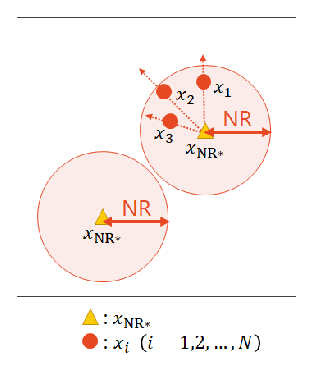
\includegraphics[width=0.4\linewidth]{eps/SICESSI2018/niche_radius.eps}
  \caption{解候補の生成}
  \label{fig:nr}
\end{figure}

局所探索では(\ref{eq:mi})式で算出した最良個体$x_{NR*}$が持つ$m_i$の範囲内で個体$x_i$が新たに解候補$x_{loc}$を生成する.
\begin{equation}
\label{eq:dnrloc}
\mbox{\boldmath $x_{loc}$}=\mbox{\boldmath $x_{NR*}$} + A_i^t*rand(1,D,[-m_i, m_i])
\end{equation}
ランダム探索では,個体$x_i$の持つ$m_i$の範囲内で新たに解候補$x_{rnd}$を生成することで,局所解への収束性能を高める.生成式は次式で表される.
\begin{equation}
\label{eq:dnrrnd}
\mbox{\boldmath $x_{rnd}$}=\mbox{\boldmath $x_i^t$} + rand(1,D,[-m_i, m_i])
\end{equation}

% アルゴリズムの疑似コードを以下に記す.

% \begin{algorithm}[H]
% \caption{Niche Radius with Bat Algorithm}
% \label{code:nrba}
% \begin{algorithmic}[1]
% \REQUIRE 評価関数 $F(x)$の設定
% \STATE 各個体$x_i(i=1,2,...,N)$と速度$v_i$の初期化
% \STATE Niche Radiusの算出 [eqs.(\ref{eq:r}), (\ref{eq:NR})]
% \STATE 周波数$f_i$の定義 [eq.(\ref{eq:freq})]
% \STATE パルスレート$r_i$とラウドネス$A_i$の初期化
% \WHILE{(t $<$ Max Iteration)}
% \IF{($d_i<NR$)}
% \STATE 新しい解$x_i^{t+1}$の生成と速度$v_i$の更新 [eqs.(\ref{eq:vi}),(\ref{eq:xi})]
% % \ELSE
% % \STATE Continue
% \ENDIF
% \IF{($rand>r_i$)}
% \STATE 生成した解$x_i^{t+1}$近辺に新しい解$x_{loc}$を生成 [eq.(\ref{eq:loc})]
% \ENDIF
% \IF{($rand<A_i \ \& \ F(x_i), F(x_{loc})>F(x_{i*})$)}
% \STATE 新しい解の評価と更新
% \STATE パルスレート$r_i$の増加とラウドネス$A_i$の減少 [eqs.(\ref{eq:loud}),(\ref{eq:pulse})]
% \ENDIF
% \ENDWHILE
% \end{algorithmic}
% \end{algorithm}

% \subsection{解候補の生成}
% 速度$v_i$を分割した解候補の中から最良の解を$x_i^{t+1}$として生成する.
\section{実験}
CEC ({\it IEEE Congress on Evolutionary Computation}) 2013 Competition 
% on Niching Methods for Multimodal Function Optimization 
\cite{CEC2013} で扱われたベンチマーク関数$G_1$-$G_6$を使用し,従来手法と比較することで提案手法の探索性能を検証する.
評価尺度として発見した解探索率Peak Ratio (PR) \cite{CEC2013} を採用し,次式で表される.
\begin{equation}
\label{eq:PR}
PR=\frac{\sum_{run=1}^{NR}NPF_{run}}{NKP*NR}
\end{equation}
$NPF_{run}$は,そのシードにおけるアルゴリズムが発見した最適解数を示し,NKPは評価関数が持つ全最適解数を示す.NRは実験の試行回数を示す.解発見の定義は最近傍個体との評価値の差分が閾値$\varepsilon$によって設定した.


本実験では$f_{max}=1$, $f_{min}=0$,ラウドネス$A^0=1$,パルスレート$r^0 \in [0,1]$と設定した.また$\alpha= \gamma = 0.9$とし,個体数$N=100$,世代数を$G_1$から$G_5$までは50000, $G_6$は200000とし,ランダムシードを変えた実験を50回行った.

\section{結果と考察}
% \begin{table}[h]
% \caption{PR値の平均及び標準偏差(実験回数50試行)}
% \begin{center}
% \begin{tabular}{c|c|c}
% \hline

% Algorithm & Median & Mean $\pm$ St.D  \\

% \hline
% NSGAII & 0.9350 & 0.7274 & 0.0646 \\
% \hline
% CMA-ES & 1.0 & 0.9371 & 0.1423 \\
% \hline
% CDE & 1.0 & 0.8229 & 0.2087 \\
% \hline
% dADE/nrand/1 & 1.0 & 0.9663 & 0.1820 \\
% \hline
% dADE/nrand/2 & 1.0 & 0.9611 & 0.1774 \\
% \hline
% DECG & 1.0 & 0.9662 & 0.1820 \\
% \hline
% DELG & 1.0 & 0.9658 & 0.1814 \\
% \hline
% DELS-aj & 1.0 & 0.9666 & 0.1825 \\
% \hline
% DE/nrand/1 & 1.0 & 0.8919 & 0.0801 \\
% \hline
% DE/nrand/2 & 1.0 & 0.9225 & 0.1221 \\
% \hline
% IPOP-CMA-ES & 0.7760 & 0.7240 & 0.0162 \\
% \hline
% NEA1 & 1.0 & 0.9166 & 0.1142 \\
% \hline
% NEA2 & 1.0 & 0.9608 & 0.1747 \\
% \hline
% N-VMO & 1.0 & 0.9540 & 0.1738 \\
% \hline
% PNA-NSGAII & 1.0 & 0.8960 & 0.0929 \\
% \hline
% NSBA & 0.6990 & 0.5953 $\pm$ 0.0629 \\
% \hline
% NRBA & 0.9520 & 0.7659 $\pm$ 0.1165 \\
% \hline
% DNRBA & 0.9070 & 0.7540 $\pm$ 0.1519 \\
% \hline

% \end{tabular}
% \label{tab:MOP_results}
% \end{center}
% \end{table}

\begin{figure}[h]
\centering
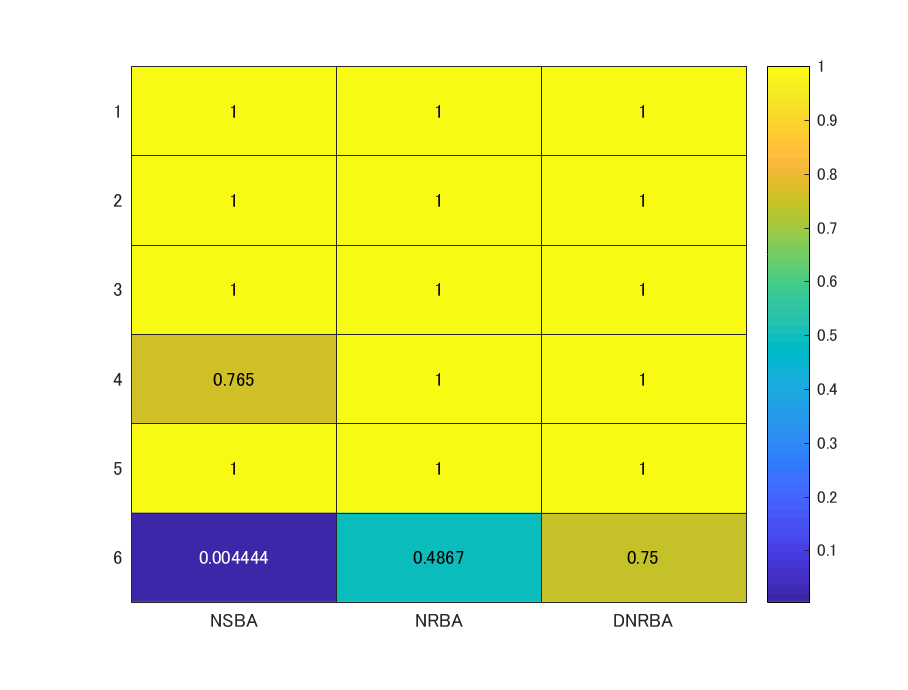
\includegraphics[width=0.7\linewidth]{eps/E-1_1.eps}
\caption{$\varepsilon=1.0E-1$におけるPRの平均値}
\label{fig:resutls_comp_E1}
\end{figure}

% \begin{figure}[t]
% \begin{center}
% \begin{tabular}{c}
% \begin{minipage}[b]{0.45\linewidth}
% \begin{center}
% 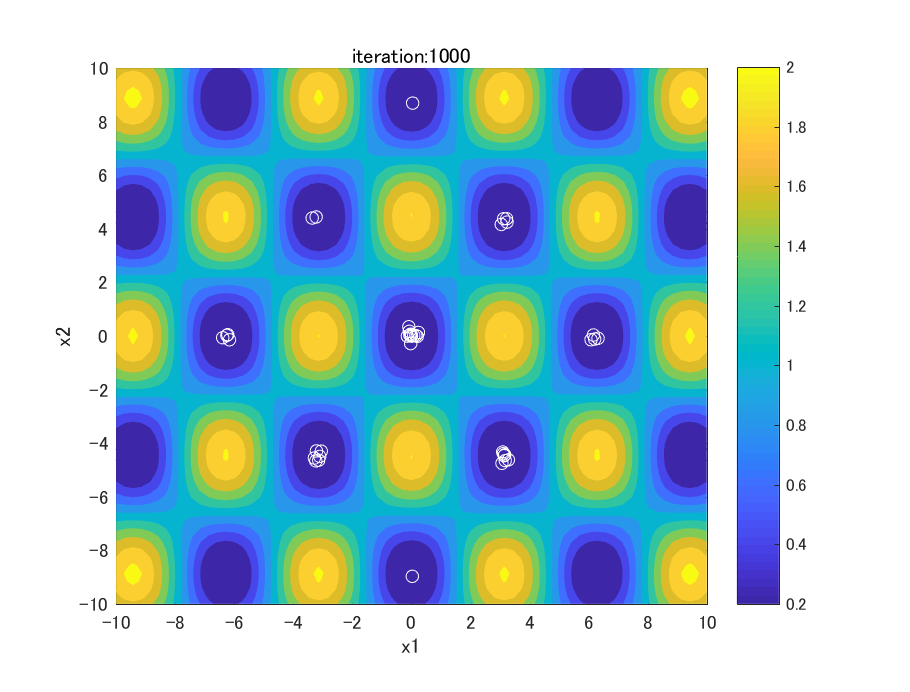
\includegraphics[keepaspectratio, scale=0.33]{eps/ba1000.eps} (i) BA

% % 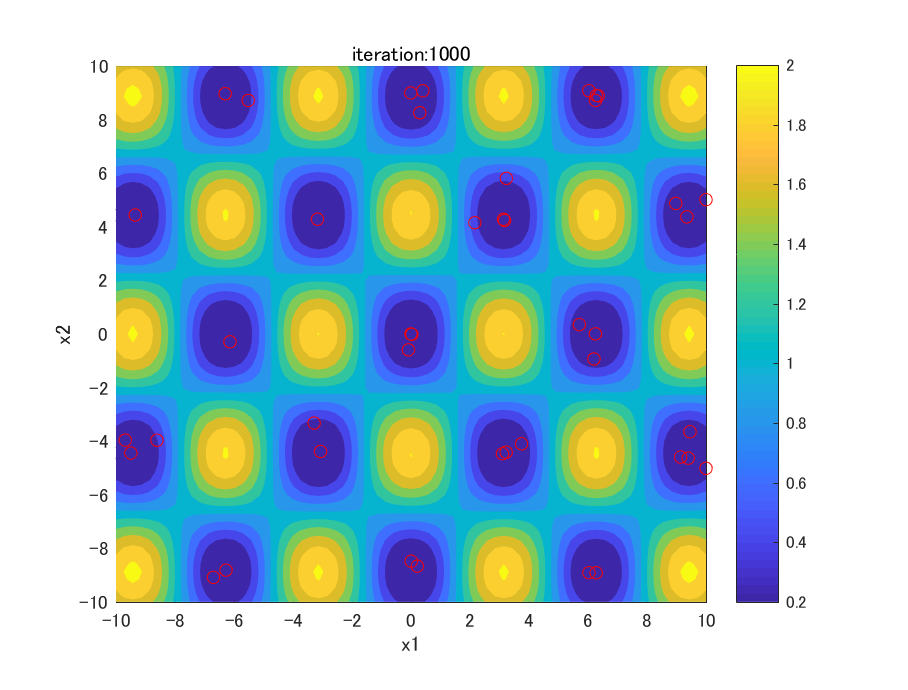
\includegraphics[width=0.8\linewidth]{eps/1000.eps}
% % \caption{1000世代目における個体の分布(NRBA)}
% % \label{fig:1000}
% \end{center}
% \end{minipage}

% \begin{minipage}[b]{0.45\linewidth}
% \begin{center}
% 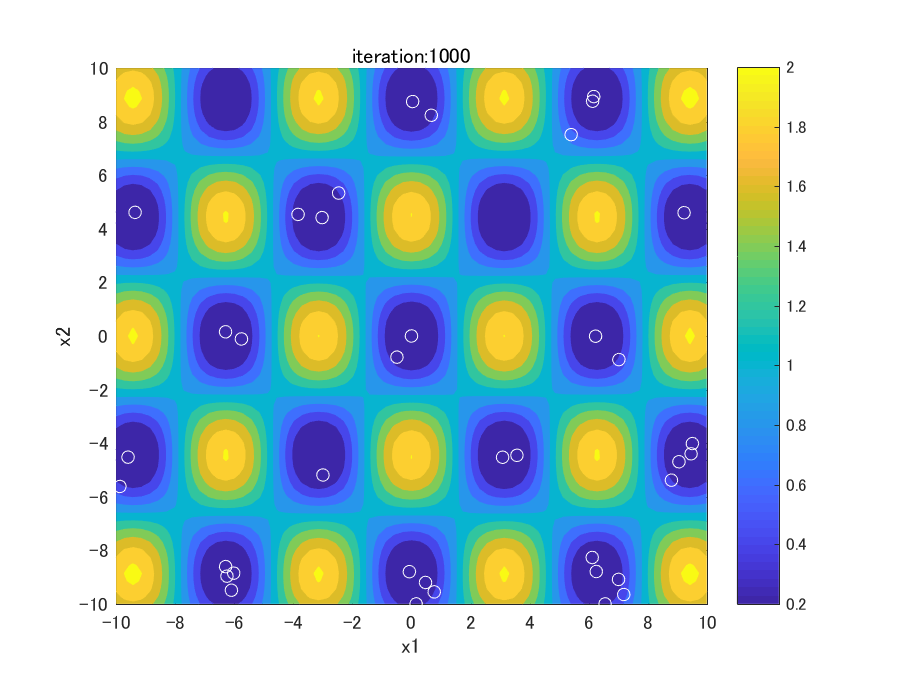
\includegraphics[keepaspectratio, scale=0.33]{eps/nrba1000.eps} (ii) NRBA
% \end{center}
% \end{minipage}
% \end{tabular}
% \caption{各手法における1000世代目の解分布}
% \label{fig:1000}
% \end{center}
% \end{figure}

図\ref{fig:resutls_comp_E1}は$\varepsilon=1.0E-1$とした時のPRの平均値をヒートマップ化したものである.
提案した3つの手法の中ではDNRBAが最もPR値が高かった.また最適解周辺の勾配が強い$G_6$関数では全ての手法で探索性能が悪化したが,中でもDNRBAは探索性能を保持することができた.これは,局所解へ陥ってしまった個体を最適解へ移動させる機構を持つDynamic Niche Radiusが複雑な関数においては有効であると考えられる.

\section{おわりに}
本研究では最適解だけでなく,複数の局所解を同時に探索可能なDNRBAを提案した.提案手法の有効性を検証するため,評価関数を用いて,他の手法との比較実験を行った.結果,複雑な多峰性を持つ関数においてはDNRBAの方が探索性能が高く,複雑な関数において有効であることを示した.
% 従来手法と比較して最適解に陥らず,複数解を探索することができた.今後の課題としては,全ての解を探索すること,実問題への適用を考慮した個体数制限下での探索性能向上を目指す.

{\small
\begin{thebibliography}{*}
\bibitem{BA} X. S. Yang, “A Metaheuristic Bat-Inspired Algorithm”, {\it in: Nature Inspired Cooperative Strategies for Optimization (NISCO 2010) (Eds J.R. Gonzalez et al.)}, {\it Studies in Com-putational Intelligence}, Springer Berlin, 284, Springer, 65-74 (2010).

% \bibitem{niche} D.Beasley, D.R. Bull, and R.R. Martin, "A sequantial niche technique for multimodal function optimization," {\it Evolutionary Computation}, vol. 1, no.2, pp. 101-125,1993.

\bibitem{CEC2013} X. Li, A. Engelbrecht, and M. G. Epitropakis, "Benchmark Functions for CEC'2013 Special Session and Competition on Niching Methods for Multimodal Function Optimization", {\it Evol. Comput.} Mach. Learn. Group, RMIT University, Melbourne, VIC, Australia, Tech. Rep., 2013.

% \bibitem{FS} D. E. Goldberg, and J. Richardson, "Genetic Algorithms with Sharing for Multimodal Function Optimization", {\it in Proc. of the Second International Conference on Genetic Algorithms}, J. Grefenstette, Ed., pp.41-49, 1987.

\bibitem{DNS} B. Miller, "Genetic algorithms with dynamic niche sharing for multimodal function optimization", {\it In: Proceedings of the IEEE International Conference on Evolutionary Computation}, 1996.
% \bibitem{crowdingDE} R. Thomsen, "Multimodal Optimization Using Crowding-Based Differential Evolution," {\it in Proc. IEEE Congr. Evol. Comput.,} pp.1382-1389, 2004.
\end{thebibliography}
}
\end{document}